
\renewcommand\appendixpagename{Anhänge}
\begin{appendices}


\chapter{Änderungen an der Parserdatei}
\begin{table}[h!]
    \centering
    \begin{tabular}{m{0.75cm}|m{4cm}|m{10cm}}
        \textbf{Zeile} & \textbf{Änderung} & \textbf{Begründung} \\
         \hline
        116 & Deklaration Kommentar & Hier wird ein mehrzeiliger Kommentar definiert, dies ist hier ein Alias für den Token \textit{JCOMMENT}\\
        \hline
        127-128 & \textit{comment} als möglicher Präfix in Klassenmember & Hier wird dem Parser mitgeteilt, dass ein Bestandteil einer Klasse wie z. B. eine Methode einen Javadoc-Kommentar besitzen kann\\
        \hline
        47 & \textit{comment} als möglicher Präfix vor Datentyp & Hier wird dem Parser mitgeteilt, dass ein Datentyp (Klasse, Schnittstelle etc. ) einen Javadoc-Kommentar haben kann \\
        \hline
        404 & Zulassung von Javadoc in Methoden & Da Javadoc-Kommentare an beliebigen Stellen auftauchen können, auch wenn es nicht empfohlen wird und keinen Mehrwert bietet, wird hier sichergestellt, dass solche Kommentare nicht zu Warnungen oder Fehler von ANTLR4 führen. Diese Javadoc-Kommentare werden nichtsdestotrotz später ignoriert.\\
        \hline
        34, 38& Zulassung von Kommentaren vor Paketdeklarationen und Imports & Hier werden Kommentare auch vor Paketdeklarationen und Import-Statements erlaubt, was vor allem bei Klassen mit Urheberrechtsangabe sinnvoll ist\\
        \hline
        105 & Zulassung von Kommentaren bei Enumerationen & Zwar werden Javadoc-Kommentare in Enumerationen mit diesem Tool nicht betrachtet, sie führen aber dennoch zu Warnungen und Fehlermeldungen. Daher werden sie hier zugelassen, aber später ignoriert. \\
        \hline
        82, 83 & Erzeugung eines separaten Knotens für \textit{Extends}- und \textit{Implements}-Deklarationen & In der originalen Version der Parserdatei wurde die Definition der Basisklasse bzw. der implementierten Schnittstellen direkt über die Tokens \textit{EXTENDS} bzw. \textit{IMPLEMENTS} gelöst. Dies wurde in einem neuen Knoten \textit{extendClass} bzw. \textit{implementInterfaces} ausgegliedert, um so das Parsing etwas zu vereinfachen.  \\
         
    \end{tabular}
    \caption{Änderungen an der Parserdatei}
    \label{tab:parser_changes}
\end{table}

\chapter{UML-Diagramm: Parser}
\begin{figure}[ht!]
    \centering
    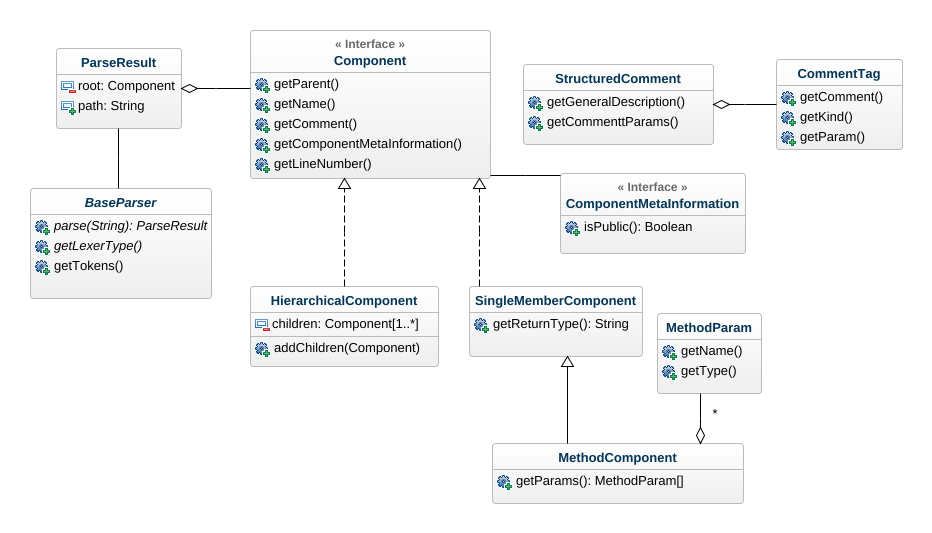
\includegraphics[height=7cm,keepaspectratio,angle=90]{figures/uml/parsing.png}
    \caption{UML-Diagramme aller Klassen, die relevant für das Parsen sind}
    \label{fig:uml_parsing}
\end{figure}
\chapter{UML-Diagramm: Metriken}
\begin{figure}[ht!]
    \centering
    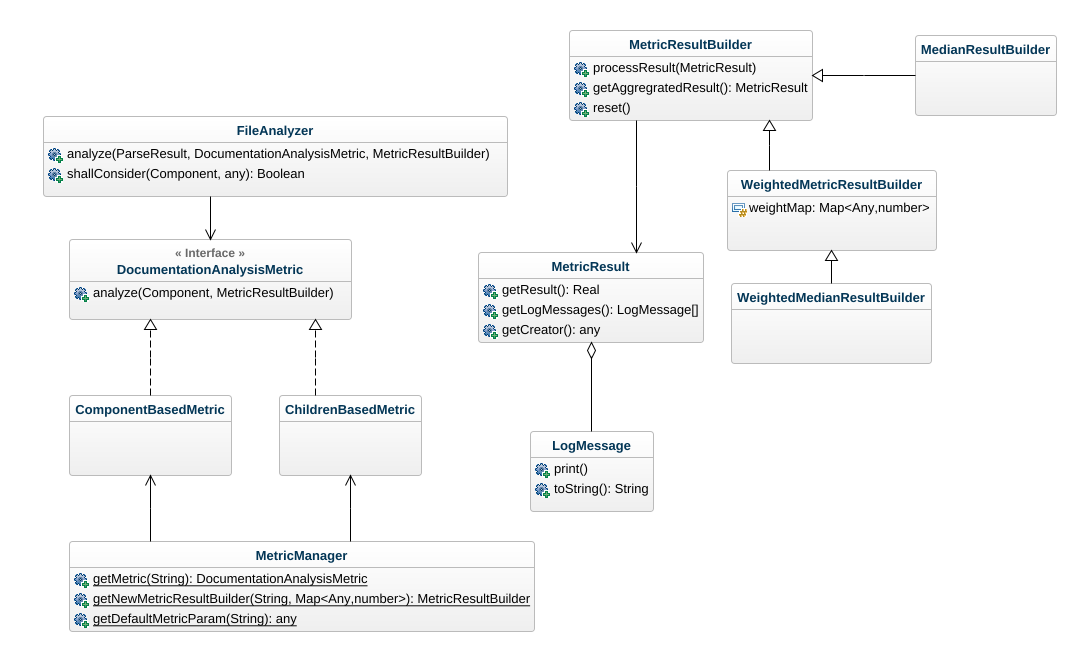
\includegraphics[height=10cm,keepaspectratio,angle=90]{figures/uml/metriken.png}
    \caption{UML-Diagramme aller Klassen, die relevant für die Metriken sind}
    \label{fig:uml_metrics}
\end{figure}
\chapter{Konfiguration des Tools}
\begin{description}
        \item[include]  Alle Dateien, die bei der Bewertung der Dokumentationsqualität berücksichtigt werden müssen
        \item[Exclude]  Teilmenge von include, enthält Dateien, die nicht weiter betrachtet werden müssen
        \item[metrics]  Alle Metriken, die das Tool verwenden soll. Dies ist ein Array von Objekten mit der Strukur \enquote{(name,weight,params)}, wobei \textit{weight} das Gewicht der jeweiligen Metrik ist( Bei Algorithmen ohne Relevanz des Gewichts wird es ignoriert), \textit{name} der Name (oder Aliasname) der Metrik und \textit{params} ein Objekt mit den Parametern der Metrik
        \item[global\_threshold] Mindestwert der Bewertung ,der erreicht werden muss, sonst wird die Dokumentationsqualität nicht akzeptiert
        \item[metric\_result\_builder] Der Name des Algorithmus/\textit{ResultBuilder}, der die einzelnen Ergebnisse der Metriken verarbeitet und so das Gesamtergebnis berechnet.
        
          \item[component\_file\_result\_builder] Der Algorithmus/\textit{ResultBuilder}, der die einzelnen Ergebnisse aller Komponenten einer Datei verarbeitet.
          
        \item[file\_result\_builder] Der Name des Algorithmus/\textit{ResultBuilder}, der die einzelnen Ergebnisse aller Dateien verarbeitet
        
        \item[parser]  Kann verwendet, um die zu parsende Programmiersprache zu wählen. Dazu muss \textit{ParserFactory} angepasst werden
        
        \item[path\_weights] Ein Array von Objekten der Struktur \enquote{(path,weight)}. Wird verwendet, um einzelne Pfade höher oder niedriger zu gewichtet
        
         \item[component\_weights] Ein Array von Objekten der Struktur \enquote{(name,weight)}. Wird verwendet, um einzelne Komponenten höher oder niedriger zu gewichtet
         
         \item[default\_path\_weight] Das Standardgewicht für eine Datei, wenn keine passende Gewichtung gefunden wurde
         
         \item[default\_component\_weight] Das Standardgewicht einer Komponente, wenn keine passende Gewichtung gefunden wurde
         
         \item[state\_manager] Kann verwendet werden, um festzulegen, wie das letzte Ergebnis der Dokumentationsqualität gespeichert werden soll. Weitere Möglichkeiten können durch Erweiterung der \textit{StateManagerFactory} hinzugefügt werden.
         
         \item[max\_diff\_last\_run] Der maximale  relative Abstand zur letzten Dokumentationsqualität bevor eine Fehlermeldung geworfen wird.
        
        
        
    \label{enum:tool_javadoc_conf}
\end{description}
\chapter{Implementierte Metriken}
\begin{table}[h!]
    \centering
    \begin{tabular}{c|c|c}
        \textbf{Metrikname} & \textbf{Klassenname} & \textbf{Erklärt in (Kapitel)}  \\\hline
          simple\_comment & SimpleCommentPresentMetric & dummy\\\hline
        public\_members\_only & SimplePublicMembersOnlyMetric &  dummy\\\hline
        large\_method\_commented & SimpleLargeMethodCommentedMetric & dummy\\\hline
     method\_fully\_documented & SimpleMethodDocumentationMetric & dummy\\\hline
       commented\_lines\_ratio& CommentedLinesRatioMetric & dummy\\\hline
       flesch& FleschMetric & dummy\\\hline
        comment\_name\_coherence&CommentNameCoherenceMetric & dummy\\\hline
     certain\_terms&CertainTermCountMetric & dummy\\\hline
          formatting\_good&FormattingGoodMetric & dummy\\\hline
          spellling&SpellingMetric & dummy\\\hline
        edge\_case&EdgeCaseMetric & dummy\\\hline
        gunning\_fog&GunningFogMetric & dummy\\
    \end{tabular}
    \caption{Alle implementierten Metriken}
    \label{table:metrics_name}
\end{table}

\end{appendices}
	
